\section{Introduction}

\begin{frame}
    \frametitle{What is hardware isolation?}

    \begin{center}
        Limiting access of software and hardware to needed resources
    \end{center}
\end{frame}

\begin{frame}
    \frametitle{Why hardware isolation?}

    \begin{center}
        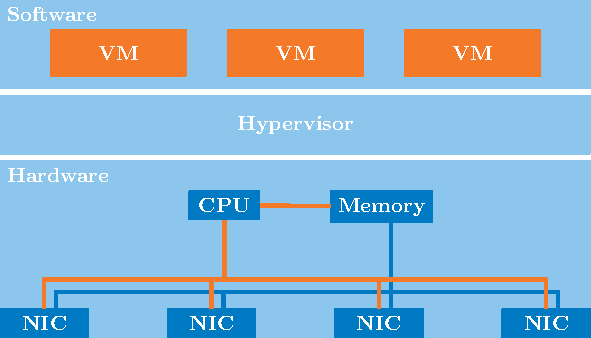
\includegraphics[width=0.9\textwidth]{figures/hypervisor-vms.pdf}
    \end{center}
\end{frame}

\begin{frame}
    \frametitle{Why hardware isolation?}

    \begin{center}
        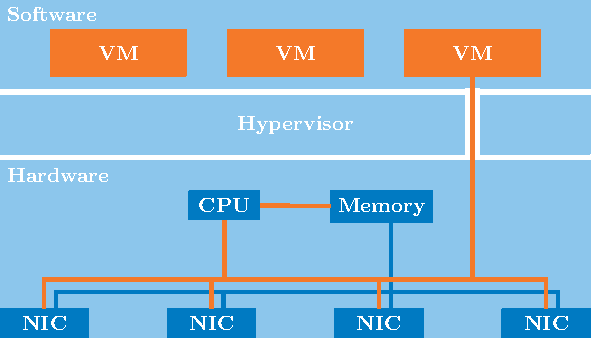
\includegraphics[width=0.9\textwidth]{figures/hypervisor-vms-pt.pdf}
    \end{center}
\end{frame}

\begin{frame}
    \frametitle{Why hardware isolation?}

    \begin{center}
        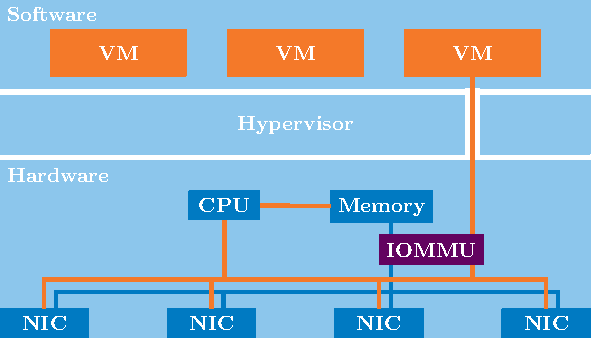
\includegraphics[width=0.9\textwidth]{figures/hypervisor-vms-pt-iommu.pdf}
    \end{center}
\end{frame}

\begin{frame}
    \frametitle{Hardware isolation via the IOMMU}
    Input-Output-Memory-Management-Unit (IOMMU):

    \begin{itemize}
        \item translates IO virtual addresses (IOVA) to physical addresses (PA)
    \end{itemize}

    \vspace{1em}
    Advantages:

    \begin{itemize}
        \item limits effects of faulty or malicious devices/software by
            restricting memory access
        \item contiguous address space does not have to be contiguous in
            physical memory
        \item enables 32-bit devices to address memory above 4 GiB
    \end{itemize}

    \vspace{1em}
    Use cases:

    \begin{itemize}
        \item virtualization
        \item vital when connecting untrusted devices via PCIe, Thunderbolt, ...
    \end{itemize}
\end{frame}

\begin{frame}
    \frametitle{Why should we look at the IOMMU?}

    Reasons to have a closer look:
    \begin{itemize}
        \item not that much information available about IOMMU implementations
        \item some publications report huge performance impacts and
            vulnerabilities
        \item implementation differences between vendors (Intel, AMD, ...)
            mostly unknown
    \end{itemize}

    \vspace{1em}
    Key question:
    \begin{itemize}
        \item What is the trade-off between performance and safety/security?
    \end{itemize}
\end{frame}

\section{Effects of the IOMMU}

\begin{frame}
    \frametitle{Performance impact}

    \begin{itemize}
        \item in non-virtualized and
        \item virtualized environments
    \end{itemize}
\end{frame}

\begin{frame}[fragile]
    \frametitle{Performance impact: Test setup}

    \begin{minipage}{0.5\textwidth}
        Performance measured with ixy.rs:

        \begin{itemize}
            \item state-of-the-art user space network driver
            \item can forward >26 million $\frac{\text{packets}}{\text{s}}$ on
                a single 3.3 GHZ CPU core
            \item less than 2,000 lines of code
            \item written in Rust
        \end{itemize}
    \end{minipage}%
    \begin{minipage}[c]{0.5\textwidth}
        \begin{figure}
            \centering
            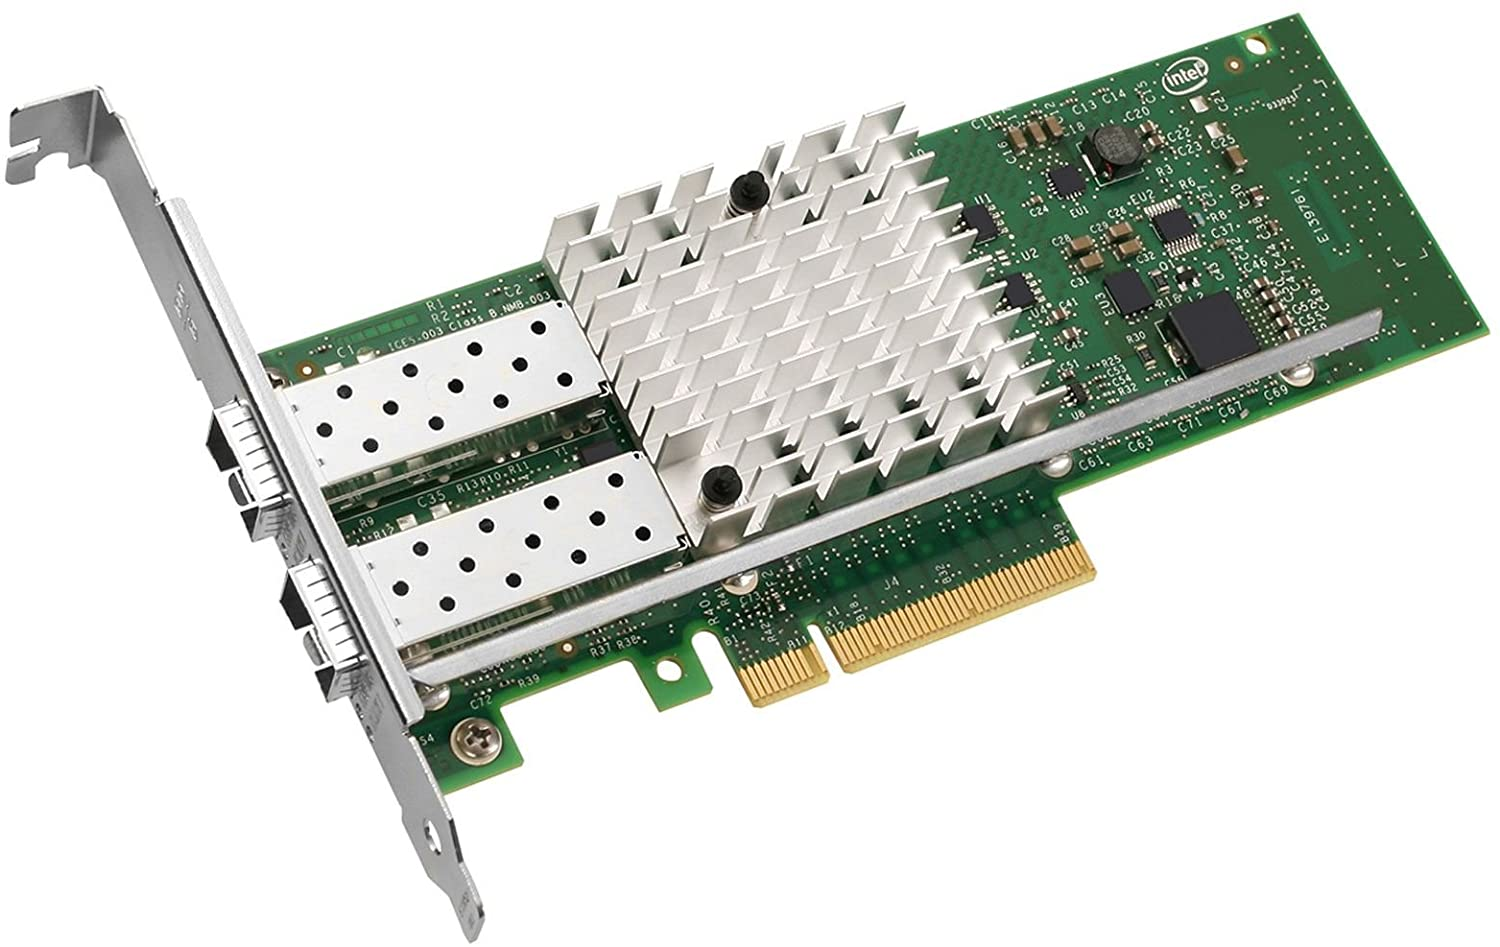
\includegraphics[width=0.8\textwidth,clip,trim=0cm 0cm 0cm
            0cm]{pics/intel_x520_da2.jpg}
            \caption{Intel X520-DA2 [Picture: amazon.com]}
        \end{figure}
    \end{minipage}
\end{frame}

\begin{frame}
    \frametitle{Performance impact: Test setup}

    \centering\includestandalone[scale=0.65]{figures/testsetup}
\end{frame}

\begin{frame}
    \frametitle{Performance impact: Test setup}

    \begin{table}
        \begin{tabular}{l | c | r | c  }
            Model                             & Clock rate & Cores & Released \\
            \hline
            Intel \hspace{0.2mm} Xeon E3-1230 v2 & 3.3 GHz & 4     & 2012     \\
            Intel \hspace{0.2mm} Xeon E5-2620 v3 & 2.4 GHz & 6     & 2014     \\
            AMD EPYC 7551P                       & 2.0 GHz & 32    & 2017
        \end{tabular}
        \caption{CPU models of device(s) under test}
    \end{table}
\end{frame}

\begin{frame}
    \frametitle{Performance impact: Baseline}

    \begin{figure}
        \centering
        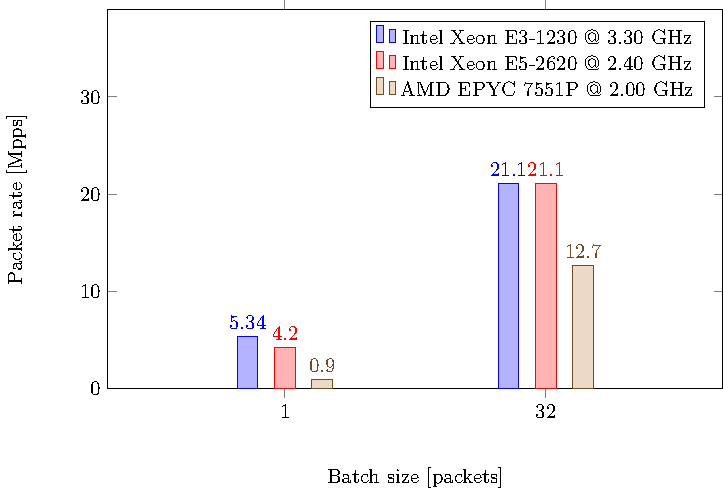
\includegraphics[width=0.8\textwidth,clip]{figures/amd-intel-perf.pdf}
        \caption{Single core forwarding rate of CPUs with different batch sizes,
        no IOMMU.}
    \end{figure}
\end{frame}

\begin{frame}
    \frametitle{Performance impact: Non-virtualized environments}

    \begin{figure}
        \centering
        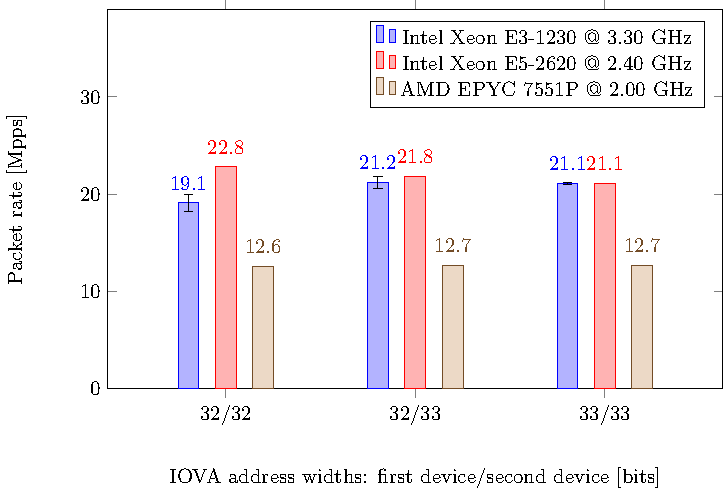
\includegraphics[width=0.8\textwidth,clip]{figures/iova-32-33-bit.pdf}
        \caption{Forwarding rate with 32 to 33 bit wide IO virtual addresses.}
    \end{figure}
\end{frame}

\begin{frame}
    \frametitle{Performance impact: Non-virtualized environments}

    \begin{figure}
        \centering
        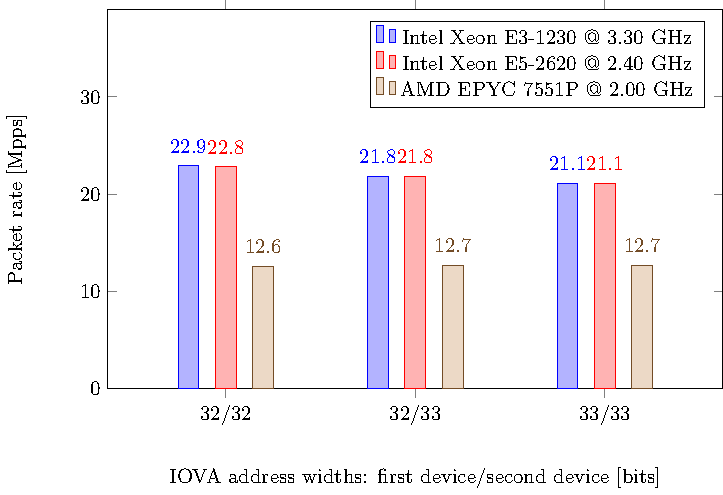
\includegraphics[width=0.8\textwidth,clip]{figures/iova-32-33-bit-queue.pdf}
        \caption{Forwarding rate with 32 to 33 bit wide IO virtual addresses,\\
        replacing the mem-pool's free-stack by a queue.}
    \end{figure}
\end{frame}

\begin{frame}
    \frametitle{Performance impact: Non-virtualized environments}

    \begin{figure}
        \centering
        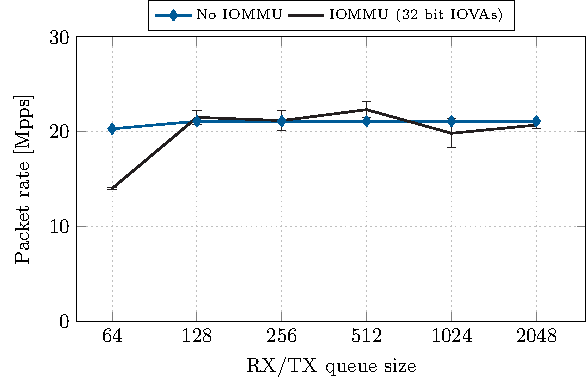
\includegraphics[width=0.8\textwidth,clip]{figures/queue-33.pdf}
        \caption{Forwarding rate of Intel Xeon E3-1230 v2 with different RX/TX
        queue sizes.}
    \end{figure}
\end{frame}

\begin{frame}
    \frametitle{Performance impact: Non-virtualized environments}

    \begin{figure}
        \centering
        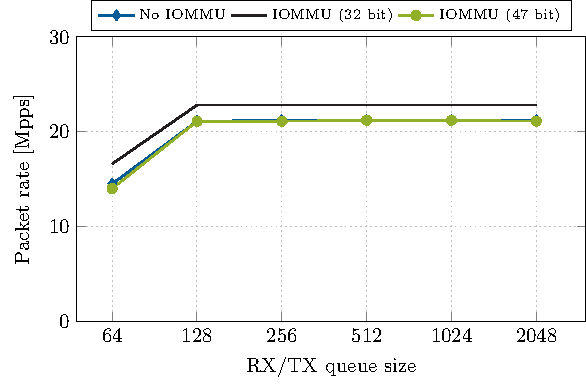
\includegraphics[width=0.8\textwidth,clip]{figures/queue-24.pdf}
        \caption{Forwarding rate of Intel Xeon E5-2620 v3 with different RX/TX
        queue sizes.}
    \end{figure}
\end{frame}

\begin{frame}
    \frametitle{Performance impact: Non-virtualized environments}

    \begin{figure}
        \centering
        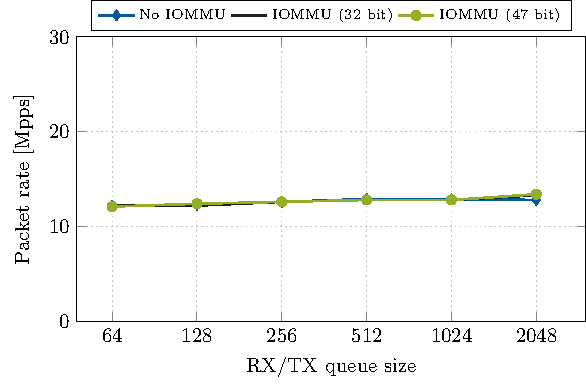
\includegraphics[width=0.8\textwidth,clip]{figures/queue-20.pdf}
        \caption{Forwarding rate of AMD EPYC 7551P with different RX/TX queue
        sizes.}
    \end{figure}
\end{frame}

\begin{frame}
    \frametitle{Performance impact: Non-virtualized environments}

    \begin{figure}
        \centering
        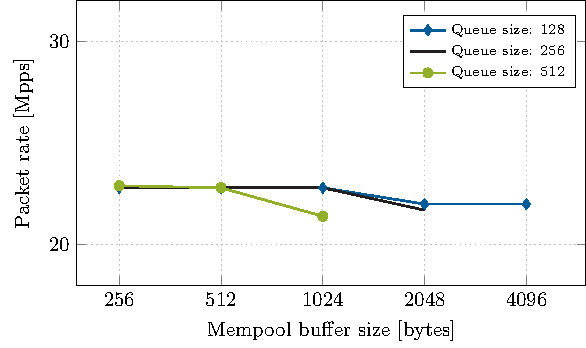
\includegraphics[width=0.8\textwidth,clip]{figures/iotlb-33.pdf}
        \caption{Forwarding rate of Intel Xeon E3-1230 v2 with 4 KB pages and
        various queue/buffer sizes.}
    \end{figure}
\end{frame}

\begin{frame}
    \frametitle{Performance impact: Non-virtualized environments}

    \begin{figure}
        \centering
        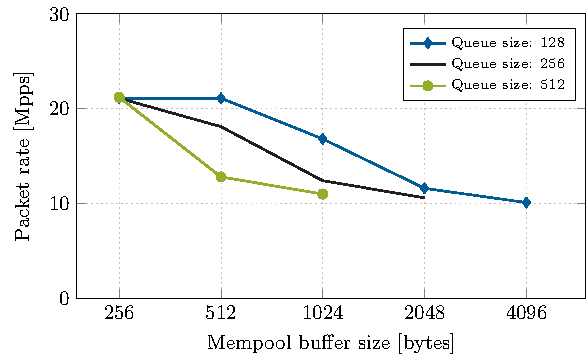
\includegraphics[width=0.8\textwidth,clip]{figures/iotlb-24.pdf}
        \caption{Forwarding rate of Intel Xeon E5-2620 v3 with 4 KB pages and
        various queue/buffer sizes.}
    \end{figure}
\end{frame}

\begin{frame}
    \frametitle{Performance impact: Non-virtualized environments}

    \begin{figure}
        \centering
        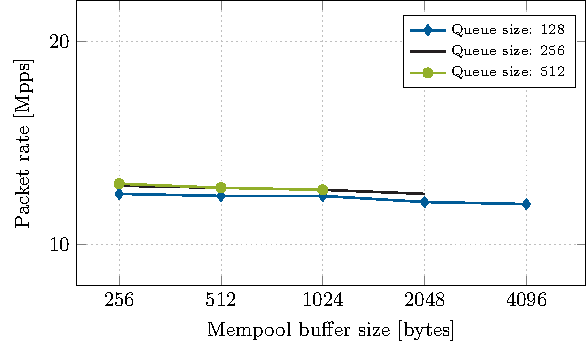
\includegraphics[width=0.8\textwidth,clip]{figures/iotlb-20.pdf}
        \caption{Forwarding rate of AMD EPYC 7551P with 4 KB pages and various
        queue/buffer sizes.}
    \end{figure}
\end{frame}

\begin{frame}
    \frametitle{Performance impact: Non-virtualized environments – Summary}

    IOMMUs may improve performance ...
    \begin{itemize}
        \item in PCIe-bottlenecked networks by using shorter (e.g. 32 bit) IO
            virtual addresses
    \end{itemize}

    \vspace{1em}
    IOMMUs may cause performance degredation ...
    \begin{itemize}
        \item when the IO-TLB gets thrashed
    \end{itemize}
\end{frame}

\begin{frame}
    \frametitle{Performance impact: Virtualized environments}

    \begin{figure}
        \centering
        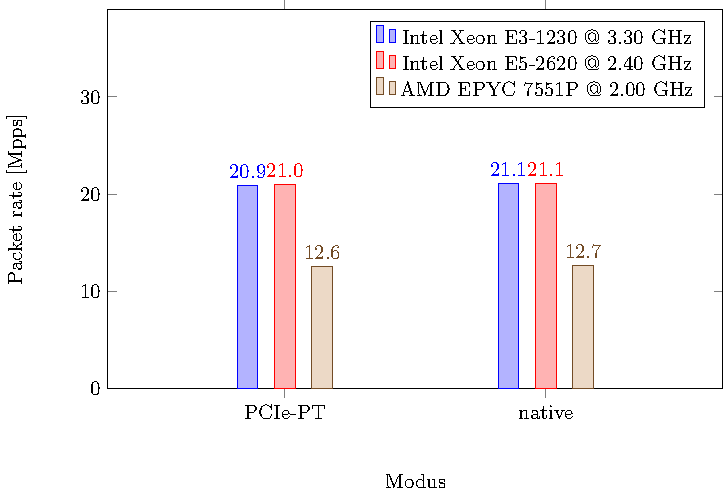
\includegraphics[width=0.8\textwidth,clip]{figures/pcie-pt.pdf}
        \caption{Forwarding rate using PCIe passthrough vs. native.}
    \end{figure}
\end{frame}

\section{Remaining research questions}

\begin{frame}
    \frametitle{Performance impact: Virtualized environments}

    \begin{center}
        To be continued
    \end{center}
\end{frame}

\section{Remaining research questions}

\begin{frame}
    \frametitle{}

    \begin{itemize}
        \item Does the IOMMU impact performance of SR-IOV or virtual switches?
        \item Are IO-TLB entries shared between multiple devices?
        \item Does the IO-TLB affect security on virtualized systems?
    \end{itemize}
\end{frame}

